\section{Conclusion}
\label{section:conclusion}
Further on this thesis will be closed with a conclusion.
Therefore, the research question: \enquote{\textit{Are Android smartphones suitable of working with \gls{see}?}} will be in focus one last time.
The research question can be interpreted into several sub questions. 
\begin{itemize}
    \item Is it possible to use \gls{see} on \gls{android} devices?
    \begin{itemize}
        \item Yes it is possible with the given implementation from chapter \ref{section:implementation}.
        The given implementation however is only a first approach and does not cover every functionality from the desktop version.
        Functions like reviewing source code are not implemented yet and need further solutions. 
    \end{itemize}
    \item Is it possible to run \gls{see} on any given \gls{android} device?
    \begin{itemize}
        \item No it is not as the results of chapter \ref{section:evaluation} show. 
        Two of the 20 participants could not attend the user study because the mobile version of \gls{see} crashed on their devices.
        18 of 20 participants however were able to use \gls{android}. 
        Five of these 18 participants reported performance issues.
        The bad performance of a device could have caused a worse result as discussed in section \ref{sec:experinece}.
        In summary, that means, in the current state of \gls{see}, an \gls{android} device with solid hardware is needed for a carefree use.
    \end{itemize}
    \item Does it make sense to use the mobile version or is the \gls{usability} too low? 
    \begin{itemize}
        \item The results discussed in section \ref{sec:usability} show that the \gls{sus}-score of the mobile version is significantly lower than the one of the desktop version.
        However, this does not have to mean that mobile version is not useful. 
        \cite{doi:10.1080/10447310802205776} provided a scale to rate the value of a \gls{sus}-score (see figure \ref{fig:sus_scale}).
        Accordingly, to Banger at al. a \gls{sus}-score below 50 means almost certainly that the product will have issues regarding \gls{usability}.
        On the other side a score between 70 and 90 is promising that the product will have a high acceptability.
        The \gls{sus}-score of the mobile version is therefore in the acceptable range even though it is significantly lower than the desktop versions score.
        It can probably be said that the mobile version is useful to have even though there is potential for improvement.
    \end{itemize}
\end{itemize}

\begin{figure}[htb]
    \centering
    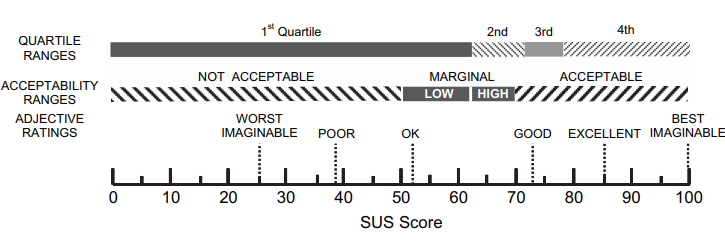
\includegraphics[width=1\textwidth]{Conclusion/img/sus.png}
    \caption{A comparison of mean System Usability Scale (SUS) scores by quartile,
    adjective ratings, and the acceptability of the overall SUS score by \cite{doi:10.1080/10447310802205776}}\label{fig:sus_scale}
  \end{figure}

  All in all the research question can be answered with \enquote{yes}.
  Regardless of the facts that the subjects needed significantly less time to solve the tasks in the user study with the desktop, the mobile version still seems to be acceptable and therefore suitable to be used.
  This can be additionally substantiated with the results from the \gls{ASQ} questionnaires, which just slightly differed between the two version.
  Also, as mentioned earlier, the \gls{sus}-score, even if significantly lower, seems to be in an acceptable range.
  It was also to expect that the outcome of a mobile version can hardly be better than the desktop version because of all the constraints a small device brings.
  The named answer of the research question is, of course, only a suggestion, since questions like these cannot be answered completely objectively.

\subsection{Further Study and Ideas}
The presented version of \gls{see} for \gls{android} devices is just a first approach and far from perfect. 
In the following ideas of improvement or further studies will be discussed.

\begin{itemize}
    \item The first thing that comes to mind is the performance of the application on certain devices. 
    Working on a small device often requires a zooming interaction.
    Zooming gets harder if the application does not run smoothly. 
    Future work could focus on improving this performance for a better user experience or at least find out what is the minimum requirement to an \gls{android} device.
    \item Some subjects mentioned concerns regarding the interface. 
    A few devices have camera notches on their display that are in the way of the menu and for other devices the joysticks were too far in the corners, so that they could not be handled properly.
    It is also thinkable that the menu could be improved in general with better icons and color.
    Improvements like these would require further user studies. 
    \item As mentioned in section \ref{sec:restructure} it was intended to restructure \gls{see} in order to minimize the need of conditional compilation.
    This process is far from trivial and would require further work. 
    \item The current version has only been tested for \gls{android} smartphones.
    It would be interesting how \gls{see} performs on tabled devices and on other operating systems like iOS.
    \item Another aspect to look at could be \gls{ar}. \cite{santos2016guidelines} provided guidelines for a mobile \gls{ar} interface, which could be adapted to \gls{see}. 
    Adding \gls{ar} to \gls{see} could have great potential and offer new innovative ways of cooperating. 
    It would also be interesting to compare the existing \gls{vr} version of \gls{see} with an \gls{ar} approach.
\end{itemize}

\subsection{Closing Words}

This thesis has started with describing the motivation and research question in chapter \ref{sec:introduction}.
To answer this question fundamental information was given in chapter \ref{sec:fundamentals} before a concept for the mobile version of \gls{see} was sketched in chapter \ref{section:concept}.
The concept was then realized almost exactly as planned in chapter \ref{section:implementation}.
It was also discussed were the implementation faced problems and how they were solved.
Then, in chapter \ref{section:evaluation}, the evaluation was planed, executed and analyzed. 
Therefore, a significance level of $\alpha = 0.05$ was used.
20 subjects participated even though only 18 could finish the user study. 
The user study gave insight on aspects like \textit{performance}, \textit{usability}, \textit{complexity} and many more.
Finally, in chapter \ref{section:conclusion} the research question was answered with \enquote{yes}, even though the answer to this question can never be completely objective and the desktop version of \gls{see} did perform better in general.